\documentclass[12pt]{standalone}

\usepackage{tikz}
\usepackage{ctex}

\begin{document}
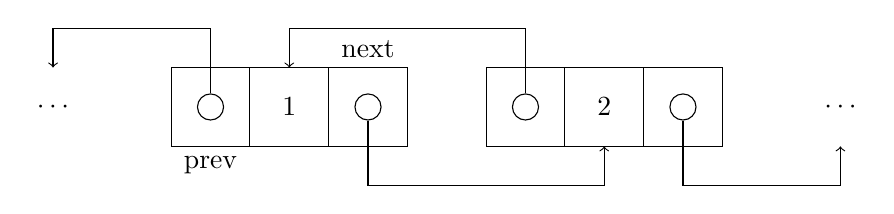
\begin{tikzpicture}

\draw
    (0,0) rectangle node[circle,draw] (A) {} (1,1)
    (1,0) rectangle node {$1$} (2,1) 
    (2,0) rectangle node[circle,draw] (B) {} (3,1);
\draw
    (4,0) rectangle node[circle,draw] (C) {} (5,1)
    (5,0) rectangle node {$2$} (6,1)
    (6,0) rectangle node[circle,draw] (D) {} (7,1);

\node at (-1.5,0.5) {$\cdots$};
\node at (8.5,0.5) {$\cdots$};

\draw[->] (A) -- ++(0,1) -- ++(-2,0) -- ++(0,-0.5);
\draw[->] (C) -- ++(0,1) -- ++(-3,0) -- ++(0,-0.5);

\draw[->] (B) -- ++(0,-1) -- ++(3,0) -- ++(0,0.5);
\draw[->] (D) -- ++(0,-1) -- ++(2,0) -- ++(0,0.5);

\node[below] at (0.5,0) {prev};
\node[above] at (2.5,1) {next};

\end{tikzpicture}
\end{document}
